%%%%%%%%%%%%%%%%%%%%%%%%%%%%%%%%%%%%%%%%%
%
%
% Modelo de Trabalho Acadêmico [UECE]
% Curso: Ciência da Computação
% Author: Luis ALves
%
% LICENSE: MIT
%
%%%%%%%%%%%%%%%%%%%%%%%%%%%%%%%%%%%%%%%%%

%----------------------------------------------------------------------------------------
%	PACOTES E CONFIGURAÇÕES DO DOCUMENTO
%----------------------------------------------------------------------------------------

\documentclass[12pt]{article} 

% Língua Brasileira e Inglesa
\usepackage[english,brazil]{babel}
\usepackage[utf8]{inputenc}

% Matemática
\usepackage{amssymb}
\usepackage{amsmath}
\usepackage{mathabx}

% Pacote para incluir imagens
\usepackage{graphicx}

% Pacote para incluir códigos
\usepackage{listings}

% Margens e paragráfos do documento
\usepackage[margin=1in]{geometry}
\setlength{\parskip}{1em}
\renewcommand{\baselinestretch}{1.5}
\setlength\parindent {0pt}

%----------------------------------------------------------------------------------------
%	CAPA DO DOCUMENTO
%----------------------------------------------------------------------------------------

\begin{document}
    
\begin{center}
    \begin{figure}
        \begin{center}
            
\includegraphics[width=0.15\textwidth]{imagens/logo_uece}
        \end{center}
    \end{figure}
    
    \title
    {
        Universidade Estadual do Ceará \\
        Centro de Ciências e Tecnologias - CCT \\
        Ciência da Computação \\
        \vspace{2.5cm}
        Lorem ipsum dolor sit amet consectetur adipiscing  \\
        \large Introdução a Ciência da Computação - 20\#\#.\#
    }
    
    \author{Fidalgo Fulano de Tal}
    \date{\today}
    \maketitle
    \newpage
\end{center}

%----------------------------------------------------------------------------------------
%	PARTE 1
%----------------------------------------------------------------------------------------

\section{Introdução}

Lorem ipsum dolor sit amet, consectetur adipiscing elit. Vestibulum maximus quam ut pellentesque accumsan. Mauris tincidunt, dolor vitae lobortis efficitur, ex ligula pharetra ipsum, at sollicitudin erat justo vitae enim. Suspendisse faucibus tincidunt rutrum. Vivamus eros justo, euismod et justo et, suscipit elementum nisl. Suspendisse potenti. Ut vitae urna vitae tellus tempus vulputate. Aliquam tellus leo, aliquet sed dolor posuere, viverra porta felis. Proin gravida ultrices imperdiet. Sed in turpis sit amet urna pretium rhoncus eget eget felis.

Sed enim nunc, condimentum sed erat at, gravida viverra enim. Morbi sed velit in ex porttitor convallis et in orci. Vivamus ultricies porta ligula, a luctus magna laoreet sed \cite{smith:99}. Nam ac ligula sit amet ipsum posuere lacinia. Sed lacinia laoreet mauris, ut consequat diam pretium a. Donec porta massa a eleifend gravida. Suspendisse nec leo luctus, maximus mauris eu, tristique diam.



\section{Formulação do Problema}

Cras vitae mi ante. Fusce fermentum, sem eget sagittis convallis, tellus ante tristique mauris, ut tincidunt nunc tellus eget purus. Donec at nulla in lectus vestibulum tristique ut ac augue \cite{sedg:11}. Curabitur sit amet nisl viverra, ultrices orci sed, accumsan justo. Integer faucibus felis ipsum, at efficitur magna hendrerit et. Morbi at sollicitudin justo, in bibendum metus. Aliquam sodales massa non rhoncus pretium:

\begin{enumerate}

\begin{item}
Lorem ipsum dolor sit amet, consectetur adipiscing elit. Vivamus in neque id neque faucibus tincidunt vel vitae felis
\end{item}

\begin{item}
Donec at nulla in lectus vestibulum tristique ut ac augue.
\end{item}

\begin{item}
Suspendisse potenti. Uta vitae urna vitae tellus tempus vulputate.
\end{item}

\end{enumerate}

\begin{figure}[h!]
    \begin{center}
    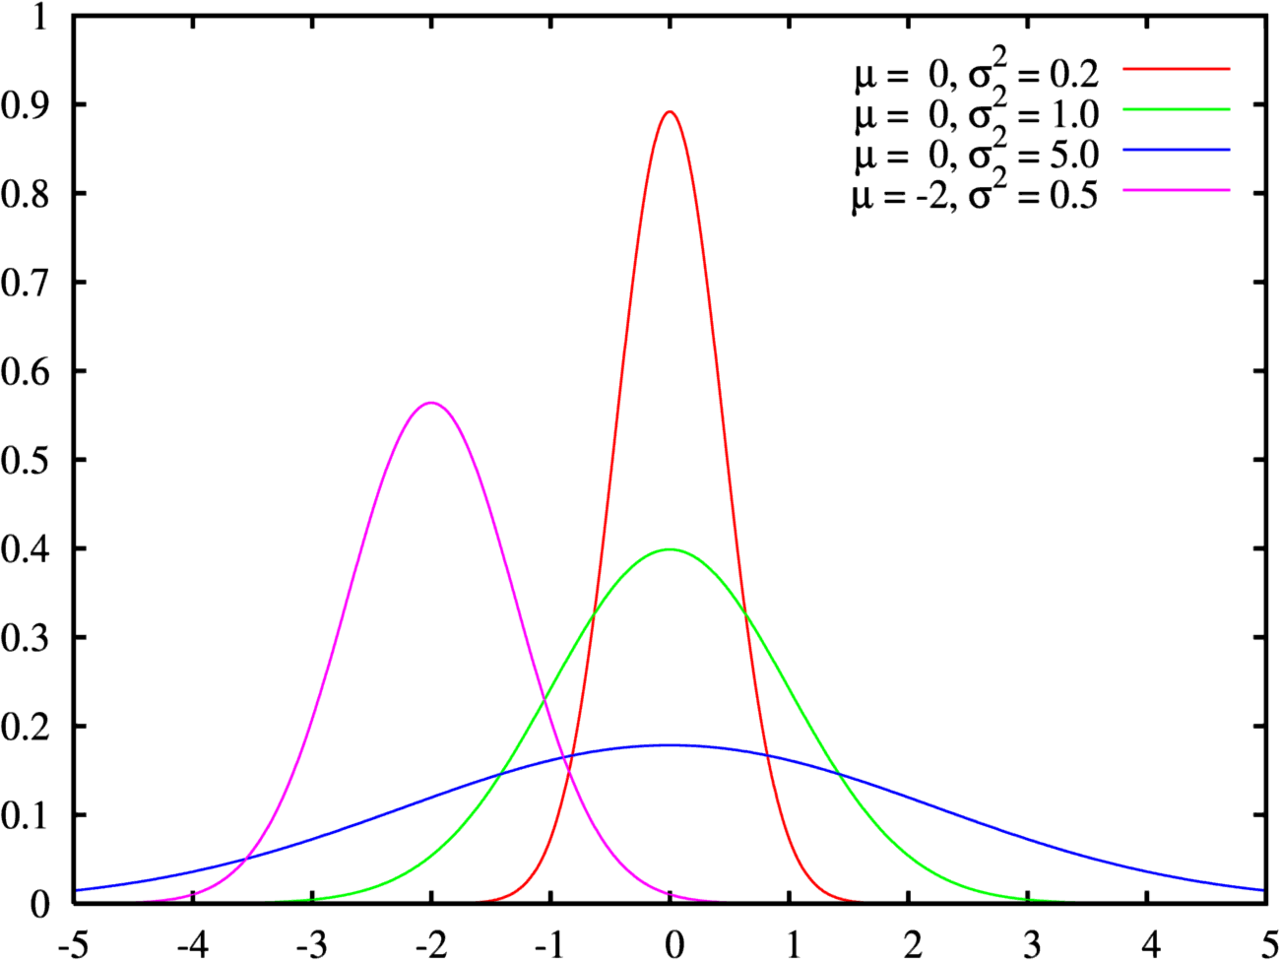
\includegraphics[width=0.60\textwidth]{imagens/gmm.png} 
    \caption{Aenean egestas turpis neque.}
    \end{center}
\end{figure}


%----------------------------------------------------------------------------------------
%	PARTE 2
%----------------------------------------------------------------------------------------

\section{Descrição do Projeto}

Nam eleifend rhoncus urna a porttitor. Nulla facilisi. Aenean egestas turpis neque, elementum commodo orci fringilla vel. Suspendisse at augue vitae ipsum tincidunt volutpat. Maecenas libero risus, euismod sed lobortis vitae, posuere cursus tortor. Nunc maximus dignissim pretium. Donec venenatis libero ullamcorper purus condimentum ultrices \cite{knuth:84}. Suspendisse ac erat nisl. Aliquam elit est, vulputate eget blandit rutrum, iaculis in velit. Maecenas orci nulla, hendrerit nec justo vitae, sodales ullamcorper enim.

In et varius purus. Etiam sem magna, tristique eu molestie sit amet, pretium a ipsum. Integer ut convallis velit. Integer pulvinar mauris non velit lobortis tincidunt. Integer in odio ut leo accumsan egestas vitae et elit. Aliquam ornare, justo vitae volutpat finibus, lectus dui consequat ex, id feugiat leo diam aliquam augue. Ut rhoncus condimentum orci quis blandit \cite{cormen:09}. Nam fermentum at nisi nec venenatis. Nullam convallis neque vel tortor feugiat, in aliquam massa placerat. Etiam accumsan vestibulum risus, at faucibus metus varius ut. Proin ultricies molestie elit, quis volutpat libero rutrum eget. Etiam porta nulla a urna sodales ultrices.




%----------------------------------------------------------------------------------------
%	PARTE 3
%----------------------------------------------------------------------------------------

\section{Descrição da Implementação}

In aliquam vehicula nisl eget fringilla. Curabitur porta lacus neque, eget tristique elit blandit quis. Nunc feugiat neque a luctus scelerisque. Cras placerat tincidunt dui laoreet consequat. Etiam risus mauris, venenatis quis ultrices vitae, commodo eget dui. Vestibulum sed facilisis massa. In sollicitudin leo a varius molestie. Praesent varius justo sed sapien lobortis, vitae aliquet arcu congue. Proin et dui sagittis, finibus orci vel, finibus turpis. Proin rutrum metus ut nisl viverra, at accumsan neque molestie. Nullam et tempor velit. Donec leo dolor, dapibus ac orci eget, aliquet pulvinar turpis.

\begin{lstlisting}[language=Python]
def dfs(self, graph, v):
    self.marked[v] = True
    for w in graph[v]:  
        if not self.marked[w]:
            self.dfs(graph, w)
            self.edge_to[w] = v
\end{lstlisting}

Vestibulum ac purus ornare, consequat neque in, hendrerit dolor. Pellentesque habitant morbi tristique senectus et netus et malesuada fames ac turpis egestas. Cras convallis ut velit ac sollicitudin. Aliquam egestas nisl sit amet risus hendrerit tristique. Nunc tincidunt, felis vel euismod laoreet, quam ligula euismod lorem, quis laoreet tortor sem tincidunt nunc. Praesent tincidunt odio in libero congue, ac dapibus sem tempus. Nam imperdiet diam sed aliquet hendrerit. Fusce id sem laoreet, ornare eros a, finibus velit. Ut in pretium urna. Aliquam odio mauris, eleifend et augue vitae, tristique bibendum erat. Phasellus congue scelerisque vehicula.


%----------------------------------------------------------------------------------------
%	PARTE 4
%----------------------------------------------------------------------------------------

\section{Resultados}

Aliquam non turpis fringilla, commodo felis vitae, egestas ex. Sed varius diam ipsum, vitae sodales sem finibus et. Nam sit amet massa fermentum, ultricies magna at, dictum eros. Interdum et malesuada fames ac ante ipsum primis in faucibus. Aenean nec erat odio. Curabitur eget scelerisque felis. Donec convallis elementum sollicitudin. Nulla et magna vitae felis molestie dignissim. Nam in justo a lorem rhoncus semper at quis sapien. Nam ultrices, massa ut sodales dictum, mi diam pharetra lectus, ac pellentesque magna lectus nec tortor. Etiam elementum mi ullamcorper tincidunt volutpat. Vestibulum ante magna, tristique et leo non, venenatis pharetra elit. Integer fringilla ex a libero elementum fringilla. Suspendisse consectetur lorem est, aliquam posuere diam imperdiet id:


\begin{table}[h!]
\begin{center}
    \begin{tabular}{r|c|c||c||c|c|c||c} \hline \hline

        $N^{\underline o}$&Instância
        & n & Início & Máxima & Média & Solução  &   Tempo(s) \\
        
        \hline
        1& Tsp10  & 10 & 3 & 193.00 & 189.00 & 181.00 &  0m0.004 \\
        
        \hline
        2& Tsp12  & 12  & 0 & 22.00 & 22.00 & 22.00 &  0m0.004s \\
        
        \hline     
        3& Tsp20 & 20 & 17 & 2516.00 & 2385.66 &  2225.00 &  0m0.014s \\
        
        \hline    
        4& Tsp29 & 29  & 4 & 2643.00 & 2554.66 & 2509.00 &  0m0.021s \\
        
        \hline
        5&  Tsp58  & 58  & 22 & 44651.00 & 44308.00 & 43867.00 &  0m0.030s \\
        
        \hline
        6& Tsp73  & 73 & 45 & 54915.00 & 54526.66 &  53782.00 &  0m0.040s \\
        
        \hline
        7& Tsp225  & 225  & 135 & 2444.00 & 2434.66 &  2430.00 &  0m0.110s \\
        
        \hline
        8& Tsp280 & 280  & 203 & 900.00 & 889.33 &  868.00 &  0m0.137s \\
        
        \hline
        
    \end{tabular}
\caption {Donec luctus id neque ac lobortis.}
\label{table:experimentos}
\end{center}
\end{table}

\subsection{Comentários sobre os resultados obtidos}

Donec luctus id neque ac lobortis. Integer pellentesque molestie vulputate. Suspendisse eu convallis lacus. In tellus tellus, euismod non auctor et, malesuada nec tortor. Aliquam erat volutpat. Proin purus urna, blandit tempor tristique ut, rutrum in nisl. Vivamus a pharetra lorem. Nunc at ultricies purus, non scelerisque elit. Mauris viverra dolor eget blandit malesuada. Duis iaculis pharetra leo, sed elementum sapien laoreet ut.

In aliquam vehicula nisl eget fringilla. Curabitur porta lacus neque, eget tristique elit blandit quis. Nunc feugiat neque a luctus scelerisque. Cras placerat tincidunt dui laoreet consequat. Etiam risus mauris, venenatis quis ultrices vitae, commodo eget dui. Vestibulum sed facilisis massa. In sollicitudin leo a varius molestie. Praesent varius justo sed sapien lobortis, vitae aliquet arcu congue. Proin et dui sagittis, finibus orci vel, finibus turpis. Proin rutrum metus ut nisl viverra, at accumsan neque molestie. Nullam et tempor velit. Donec leo dolor, dapibus ac orci eget, aliquet pulvinar turpis.


\section{Conclusão}

Vestibulum ac purus ornare, consequat neque in, hendrerit dolor. Pellentesque habitant morbi tristique senectus et netus et malesuada fames ac turpis egestas. Cras convallis ut velit ac sollicitudin. Aliquam egestas nisl sit amet risus hendrerit tristique. Nunc tincidunt, felis vel euismod laoreet, quam ligula euismod lorem, quis laoreet tortor sem tincidunt nunc. Praesent tincidunt odio in libero congue, ac dapibus sem tempus. Nam imperdiet diam sed aliquet hendrerit. Fusce id sem laoreet, ornare eros a, finibus velit. Ut in pretium urna. Aliquam odio mauris, eleifend et augue vitae, tristique bibendum erat. Phasellus congue scelerisque vehicula.


\bibliographystyle{cite}
\bibliography{sbc-cite}

\end{document}
